% questions.tex —— 1991 年·三南卷 · 题目内容片段（无答案）
% 由 tools/generate_projects.py 依来源总账自 1991/1991_数学真题_三南_试题.md 生成，勿手改（改源 MD 后重跑）


\gkpart{试题}

\begin{gktip}
\textbf{来源说明}：固定来源文件为普通高考/1991/1991三南(湖南,海南,云南).pdf，原页标题为“1991 普通高等学校招生考试（三南卷）”。一页 A3 横向排印稿，印刷页码 41，含第 1—30 题及两幅题图；原件未附答案、解析、分值或文理科标注。以下按原页转录，图稿为独立 TikZ 源。

\textbf{待核说明}：第 28 题原文末句缺少“求”等动词，原样保留。第 29 题原文未指定坐标系、中心或焦轴方向，后续解析须明确坐标选择，不得把选择的坐标条件冒充题设。
\end{gktip}

\AddToHookNext{file/questions.tex/after}{\clearpage}

\begin{question}
\gkti{1}

$\sin15^\circ\cos30^\circ\sin75^\circ$ 的值等于\mbox{（　　）}

（A）$\dfrac{\sqrt3}4$　　（B）$\dfrac{\sqrt3}8$　　（C）$\dfrac18$　　（D）$\dfrac14$

\end{question}
\begin{question}
\gkti{2}

已知一个等差数列的第 5 项等于 10，前 3 项的和等于 3，那么\mbox{（　　）}

（A）它的首项是 $-2$，公差是 3　　（B）它的首项是 2，公差是 $-3$

（C）它的首项是 $-3$，公差是 2　　（D）它的首项是 3，公差是 $-2$

\end{question}
\begin{question}
\gkti{3}

设正六棱锥的底面边长为 1，侧棱长为 $\sqrt5$，那么它的体积为\mbox{（　　）}

（A）$6\sqrt3$　　（B）$2\sqrt3$　　（C）$\sqrt3$　　（D）2

\end{question}
\begin{question}
\gkti{4}

\Needspace{5\baselineskip}
在直角坐标系 $xOy$ 中，参数方程
\nopagebreak[4]
\[
\begin{cases}
x=2t+1,\\
y=2t^2-1
\end{cases}
\]
（其中 $t$ 是参数）表示的曲线是\mbox{（　　）}

（A）双曲线　　（B）抛物线　　（C）直线　　（D）圆

\end{question}
\begin{question}
\gkti{5}

设全集为自然数集 $\mathbb N$，$E=\{x\mid x=2n,\ n\in\mathbb N\}$，$F=\{x\mid x=4n,\ n\in\mathbb N\}$，那么集合 $\mathbb N$ 可以表示成\mbox{（　　）}

（A）$E\cap F$　　（B）$\overline E\cup F$　　（C）$E\cup\overline F$　　（D）$\overline E\cap\overline F$

\end{question}
\begin{question}
\gkti{6}

已知 $z_1,z_2$ 是两个给定的复数，且 $z_1\ne z_2$，它们在复平面上分别对应于点 $Z_1$ 和点 $Z_2$。如果 $z$ 满足方程 $|z-z_1|-|z-z_2|=0$，那么 $z$ 对应的点 $Z$ 的集合是\mbox{（　　）}

（A）双曲线　　（B）线段 $Z_1Z_2$ 的垂直平分线

（C）分别过 $Z_1,Z_2$ 的两条相交直线　　（D）椭圆

\end{question}
\begin{question}
\gkti{7}

设 $5\pi<\theta<6\pi$，$\cos\dfrac\theta2=a$，那么 $\sin\dfrac\theta4$ 等于\mbox{（　　）}

（A）$-\dfrac{\sqrt{1+a}}2$　　（B）$-\dfrac{\sqrt{1-a}}2$　　（C）$-\sqrt{\dfrac{1+a}2}$　　（D）$-\sqrt{\dfrac{1-a}2}$

\end{question}
\begin{question}
\gkti{8}

函数 $y=\sin x$，$x\in\left[\dfrac\pi2,\dfrac{3\pi}2\right]$ 的反函数为\mbox{（　　）}

（A）$y=\arcsin x$，$x\in[-1,1]$　　（B）$y=-\arcsin x$，$x\in[-1,1]$

（C）$y=\pi+\arcsin x$，$x\in[-1,1]$　　（D）$y=\pi-\arcsin x$，$x\in[-1,1]$

\end{question}
\begin{question}
\gkti{9}

复数 $z=-3\left(\sin\dfrac43\pi-\mathrm i\cos\dfrac43\pi\right)$ 的辐角的主值是\mbox{（　　）}

（A）$\dfrac43\pi$　　（B）$\dfrac53\pi$　　（C）$\dfrac{11}6\pi$　　（D）$\dfrac\pi6$

\end{question}
\begin{question}
\gkti{10}

满足 $\sin\left(x-\dfrac\pi4\right)\ge\dfrac12$ 的 $x$ 的集合是\mbox{（　　）}

（A）$\left\{x\mid 2k\pi+\dfrac5{12}\pi\le x\le2k\pi+\dfrac{13}{12}\pi,\ k\in\mathbb Z\right\}$

（B）$\left\{x\mid 2k\pi-\dfrac\pi{12}\le x\le2k\pi+\dfrac7{12}\pi,\ k\in\mathbb Z\right\}$

（C）$\left\{x\mid 2k\pi+\dfrac\pi6\le x\le2k\pi+\dfrac56\pi,\ k\in\mathbb Z\right\}$

（D）$\left\{x\mid 2k\pi\le x\le2k\pi+\dfrac\pi6\ \text{\text{或}}\ 2k\pi+\dfrac56\pi\le x\le(2k+1)\pi,\ k\in\mathbb Z\right\}$

\end{question}
\begin{question}
\gkti{11}

点 $(4,0)$ 关于直线 $5x+4y+21=0$ 的对称点是\mbox{（　　）}

（A）$(-6,8)$　　（B）$(-8,-6)$　　（C）$(6,8)$　　（D）$(-6,-8)$

\end{question}
\begin{question}
\gkti{12}

极坐标方程 $4\sin2\theta=3$ 表示的曲线是\mbox{（　　）}

（A）二条射线　　（B）二条相交直线　　（C）圆　　（D）抛物线

\end{question}
\begin{question}
\gkti{13}

由数字 $0,1,2,3,4,5$ 组成无重复数字的六位数，其中个位数字小于十位数字的共有\mbox{（　　）}

（A）210 个　　（B）300 个　　（C）464 个　　（D）600 个

\Needspace{0.4\textheight}
\end{question}
\begin{question}
\gkti{14}

如图是周期为 $2\pi$ 的三角函数 $y=f(x)$ 的图象，那么 $f(x)$ 可以写成\mbox{（　　）}
\nopagebreak[4]
\begin{center}% 来源：1991三南原卷，PDF第1页（印刷页41），第14题。
% 数学化重建：按原图周期、幅值、x=1处下降过零及给定选项使用sin(1-x)。
% 保留原图的坐标标号和虚线；不增加未给出的刻度或题设条件。
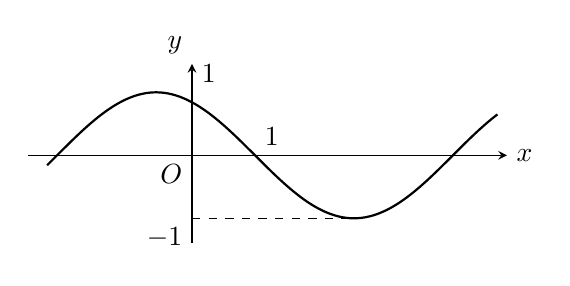
\begin{tikzpicture}[x=0.8cm,y=0.8cm,>=stealth]
  \draw[->] (-2.6,0)--(5,0) node[right] {$x$};
  \draw[->] (0,-1.4)--(0,1.45) node[above left] {$y$};
  \node[below left] at (0,0) {$O$};
  \node[above right] at (0,1) {$1$};
  \node[below left] at (0,-1) {$-1$};
  \node[above right] at (1,0) {$1$};
  \draw[dashed] (0,-1)--({1+pi/2},-1);
  \draw[thick,domain=-2.3:4.85,samples=120,smooth]
    plot (\x,{sin((1-\x) r)});
\end{tikzpicture}
\end{center}
\nopagebreak[4]
（A）$\sin(1+x)$　　（B）$\sin(-1-x)$　　（C）$\sin(x-1)$　　（D）$\sin(1-x)$

\end{question}
\begin{question}
\gkti{15}

设命题甲为 $\lg x^2=0$；命题乙为 $x=1$。那么\mbox{（　　）}

（A）甲是乙的充分条件，但不是乙的必要条件

（B）甲是乙的必要条件，但不是乙的充分条件

（C）甲是乙的充要条件

（D）甲不是乙的充分条件，也不是乙的必要条件

\end{question}
\begin{question}
\gkti{16}

$\left(\sqrt x-\dfrac2{\sqrt x}\right)^6$ 的展开式中常数项是\mbox{（　　）}

（A）$-160$　　（B）$-20$　　（C）20　　（D）160

\end{question}
\begin{question}
\gkti{17}

体积相等的正方体、球、等边圆柱（即底面直径与母线相等的圆柱）的全面积分别为 $S_1,S_2,S_3$，那么它们的大小关系为\mbox{（　　）}

（A）$S_1<S_2<S_3$　　（B）$S_1<S_3<S_2$　　（C）$S_2<S_3<S_1$　　（D）$S_2<S_1<S_3$

\end{question}
\begin{question}
\gkti{18}

曲线 $2y^2+3x+3=0$ 与曲线 $x^2+y^2-4x-5=0$ 的公共点的个数是\mbox{（　　）}

（A）4　　（B）3　　（C）2　　（D）1

\end{question}
\begin{question}
\gkti{19}

椭圆 $9x^2+16y^2=144$ 的离心率为\underline{\hspace{6em}}。

\end{question}
\begin{question}
\gkti{20}

设复数 $z_1=2-\mathrm i$，$z_2=1-3\mathrm i$，则复数 $\dfrac{\mathrm i}{z_1}+\dfrac{\overline{z_2}}5$ 的虚部等于\underline{\hspace{6em}}。

\end{question}
\begin{question}
\gkti{21}

已知圆台的上、下底面半径分别为 $r,2r$，侧面积等于上、下底面积之和，则圆台的高为\underline{\hspace{6em}}。

\end{question}
\begin{question}
\gkti{22}

$\displaystyle\lim_{n\to\infty}\dfrac{4n\cdot2^n+1}{n\cdot3^n-1}=$\underline{\hspace{6em}}。

\end{question}
\begin{question}
\gkti{23}

在体积为 $V$ 的斜三棱柱 $ABC-A'B'C'$ 中，已知 $S$ 是侧棱 $CC'$ 上的一点，过点 $S,A,B$ 的截面截得的三棱锥的体积为 $V_1$，那么过点 $S,A',B'$ 的截面截得的三棱锥的体积为\underline{\hspace{6em}}。

\end{question}
\begin{question}
\gkti{24}

设函数 $f(x)=x^2+x+\dfrac12$ 的定义域是 $\{n,n+1\}$（$n$ 是自然数），那么在 $f(x)$ 的值域中共有\underline{\hspace{4em}}个整数。

\end{question}
\begin{question}
\gkti{25}

已知 $\alpha,\beta$ 为锐角，$\cos\alpha=\dfrac45$，$\tan(\alpha-\beta)=\dfrac13$，求 $\cos\beta$ 的值。

\end{question}
\begin{question}
\gkti{26}

解不等式：$\sqrt{5-4x-x^2}\ge x$。

\Needspace{0.4\textheight}
\end{question}
\begin{question}
\gkti{27}

如图，已知直棱柱 $ABC-A_1B_1C_1$ 中，$\angle ACB=90^\circ$，$\angle BAC=30^\circ$，$BC=1$，$AA_1=\sqrt6$，$M$ 是 $CC_1$ 的中点。求证：$AB_1\perp A_1M$。
\nopagebreak[4]
\begin{center}% 来源：1991三南原卷，PDF第1页（印刷页41），第27题。
% 忠实复现投影中的连接与虚实线；平面投影位置不表示额外的度量条件。
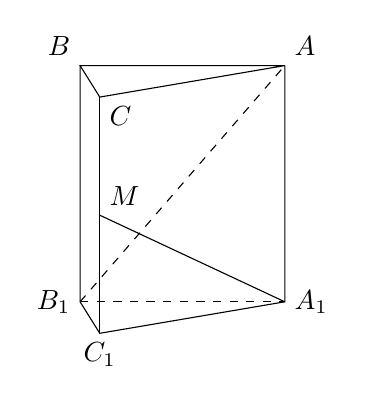
\begin{tikzpicture}[scale=1.0]
  \coordinate (B) at (0,3);
  \coordinate (A) at (2.6,3);
  \coordinate (C) at (0.25,2.6);
  \coordinate (B1) at (0,0);
  \coordinate (A1) at (2.6,0);
  \coordinate (C1) at (0.25,-0.4);
  \coordinate (M) at (0.25,1.1);
  \draw (B)--(A)--(C)--cycle;
  \draw (B)--(B1)--(C1)--(A1)--(A);
  \draw (C)--(C1);
  \draw (M)--(A1);
  \draw[dashed] (B1)--(A1);
  \draw[dashed] (B1)--(A);
  \node[above left] at (B) {$B$};
  \node[above right] at (A) {$A$};
  \node[below right] at (C) {$C$};
  \node[left] at (B1) {$B_1$};
  \node[right] at (A1) {$A_1$};
  \node[below] at (C1) {$C_1$};
  \node[above right] at (M) {$M$};
\end{tikzpicture}
\end{center}
\nopagebreak[4]
\end{question}
\begin{question}
\gkti{28}设 $\{a_n\}$ 是等差数列，$a_1=1$，$S_n$ 是它的前 $n$ 项和；$\{b_n\}$ 是等比数列，其公比的绝对值小于 1，$T_n$ 是它的前 $n$ 项和，如果 $a_3=b_2$，$S_5=2T_2-6$，$\displaystyle\lim_{n\to\infty}T_n=9$，$\{a_n\},\{b_n\}$ 的通项公式。

\end{question}
\begin{question}
\gkti{29}已知双曲线 $C$ 的实半轴长与虚半轴的乘积为 $\sqrt3$，$C$ 的两个焦点分别为 $F_1,F_2$，直线 $l$ 过 $F_2$ 且与直线 $F_1F_2$ 的夹角为 $\tan\varphi=\dfrac{\sqrt{21}}2$，$l$ 与线段 $F_1F_2$ 的垂直平分线的交点是 $P$，线段 $PF_2$ 与双曲线 $C$ 的交点为 $Q$，且 $|PQ|:|QF_2|=2:1$。求双曲线 $C$ 的方程。

\end{question}
\begin{question}
\gkti{30}已知函数 $f(x)=\dfrac{2^x-1}{2^x+1}$。

（1） 证明：$f(x)$ 在 $(-\infty,+\infty)$ 上是增函数；

（2） 证明：对于任意不小于 3 的自然数 $n$，都有 $f(n)>\dfrac n{n+1}$。

\end{question}